\documentclass[]{report}
\usepackage{pdfpages}
%\usepackage{amsmath}
\begin{document}
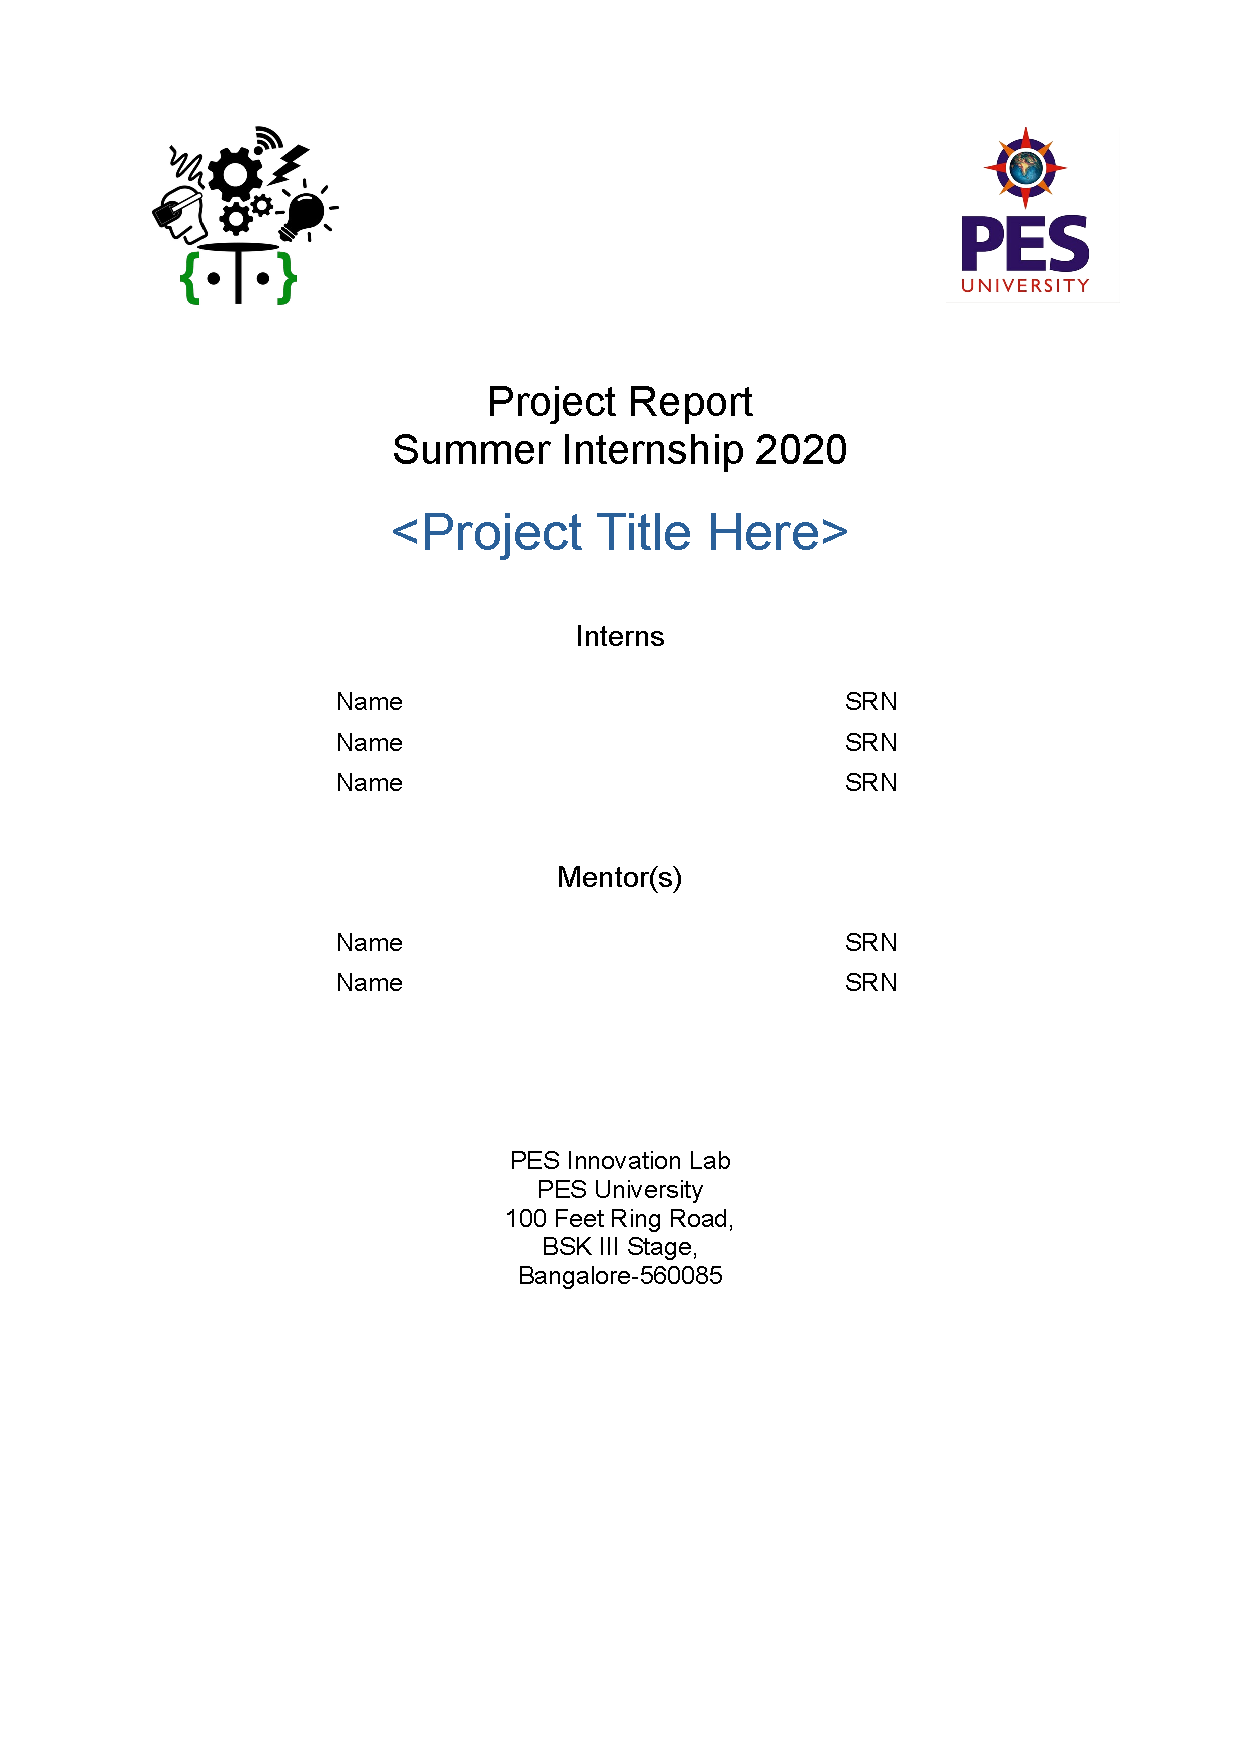
\includepdf[pages={1}]{coverpage.pdf} 

\begin{abstract}
 The recent few years, significant increase in air pollution have routinely caused panic and are a major topic of discussion by the public and air pollution experts in government and academia. There is no doubt that the keeping the air quality clean and protect it from various sources of emissions represents a major global issues and concern for any government . Quality of urban environment directly affects people health, and it is important to understand the real-time status of urban air quality. AQVis aims to successfully visualize the Air Quality Data Produced by the sensors via Cloud and get Meaningful Visualization from the data.This report on AQVis aims to design and implement a framework based cloud management system that efficiently visualizes the data that is brought from the sensors.
\end{abstract}

\tableofcontents
%\listoffigures
%\listoftables

\chapter{Introduction}
\section{Background}
Students and faculty from PES University are working on developing Air Quality sensors that can be used to detect the particulate matter concentration around where they are placed. These devices will have three individual sensors, each detecting the count of particulate matter that are 2.5, 7.5 and 10 micrometers or less in diameter. These devices will send the data obtained by the sensors to a cloud based system along with other information such as battery level, location and the timestamp.
\section{Problem Statement}
This project aims to be the cloud based counterpart of the Air Quality sensors. Cloud based servers must be able to ingest the data sent by the devices and store it in a secure and accessible manner. A dashboard created must house relevant visualizations and maps to generate useful insights from the data.
\section{Application}
The cloud based system and dashboard will be used to convey information about air quality to users. Currently, there very limited air quality sensors in India. This project aims to make sensors more widespread to enable the accurate tracking of air pollution parameters. Using this data, insights can be gained on the effect of external factors on pollution and trends in particulate matter concentration.

 

\chapter{Literature Survey/Related Work} 
\section{Existing Solutions}
There are multiple online air quality monitoring websites that we have referred to throughout the course of this project.

\subsection{PurpleAir}
PurpleAir\cite{purpleair} is a brand of air quality sensors that can be purchased and installed at any location. They connect to the server via wifi and monitor multiple different sizes of particulate matter. The online dashboard of PurpleAir shows a map with a point at the location of each sensor. The point displays a color according to the health safety and a number corresponding to an average sensor measurement. The map can be interacted with to locate different sensors. Upon clicking on a sensor, a graph displaying data from that sensor is displayed. We found this user interface very easy to use and have used it as a reference in our final design.

\subsection{Aqandu}
Aquandu\cite{aqandu} is an air quality monitoring dashboard that procures data from already placed sensors. It has been created by researchers at the University of Utah and centres the data around Salt Lake City. The data on Aquandu is sourced from four different types of sensors. The map is in black and white and a fixed graph with the data from the selected sensor is displayed at the bottom. The University of Utah has also used the data accumulated to model and forecast pollution data.\cite{aqandu:mlvideo} Attempting something similar to this is part of the future scope for this our project.

\section{Novelty of Work}
The solution we are developing is similar to the above mentioned examples in the basic approach. A map along with graphs for the selected sensors will be prominently displayed on our web page. A unique feature that we are working on that sets this solution apart from is the presence of moving sensors. Having sensors that constantly change their location results in a larger number of variables and unique computations to visualize information. This feature has not been implemented in the above mentioned solutions. Having a custom built server and dashboard will allow greater autonomy over the processing and storage of data along with better control over data analysis. Parameters and functions can be instantly tweaked according to the sensor's evolving capabilities which is difficult to accomplish with an existing solution.

\chapter{Approach}
After research and trial, the approach we decided on was to develop an API server using Flask to handle the incoming requests from the sensor devices. The ELK stack comprising of Elasticsearch, Logstash and Kibana is used to handle and visualize the data. Elasticsearch is used as the database and Kibana is used to visualize the data. OpenLayers is used to generate maps. A custom dashboard was built consisting of the graphs from Kibana and OpenLayers maps that will face the user. Using Kibana for the graphs allows them to be dynamic and easily modifiable which results in users being able to tweak the views to their specifications. The flow of data from sensors to the users is depicted in Figure \ref{dataflow}. Message Queues are a feature we expect to add in the future to reduce the load on our server and streamline data ingestion. All the software used in this project was hosted on virtual machines using Google Cloud Platform.

\section{Database}
One of the most pivotal parts to this project is the logging of data that is received from the sensors. This calls for a database management system that will suit this need accordingly. There are two major classifications when it comes to database selection .viz SQL based and NoSQL based.

SQL Based
Relational databases store data sets as “relations”: tables with rows and columns where all information is stored as a value of a specific cell. Data in an RDBMS is managed using SQL. Though there are different implementations, SQL is standardized and provides a level of predictability and utility.
Relational databases excel at handling highly structured data and provide support for ACID (Atomicity, Consistency, Isolation, and Durability) transactions. Data is easily stored and retrieved using SQL queries
The biggest weakness of relational databases is the mirror of their biggest strength. As good as they are at handling structured data, they have a hard time with unstructured data.

No SQL based
Even though many sites use an SQL database for logging, it’s not really the most efficient place to store data from a logging workload. Logs don’t require UPDATE/DELETE or rollback, they’re basically an append-only workload. So using a database engine that is designed to support OLTP workload is missing an opportunity to use a more specialized storage solution. Thus taking all this into account, logstash seemed to be the best fit for the need at hand. Logstash is available as a part of ELK stack or Elastic stack which is explained in further sections.

\begin{figure}[ht]
  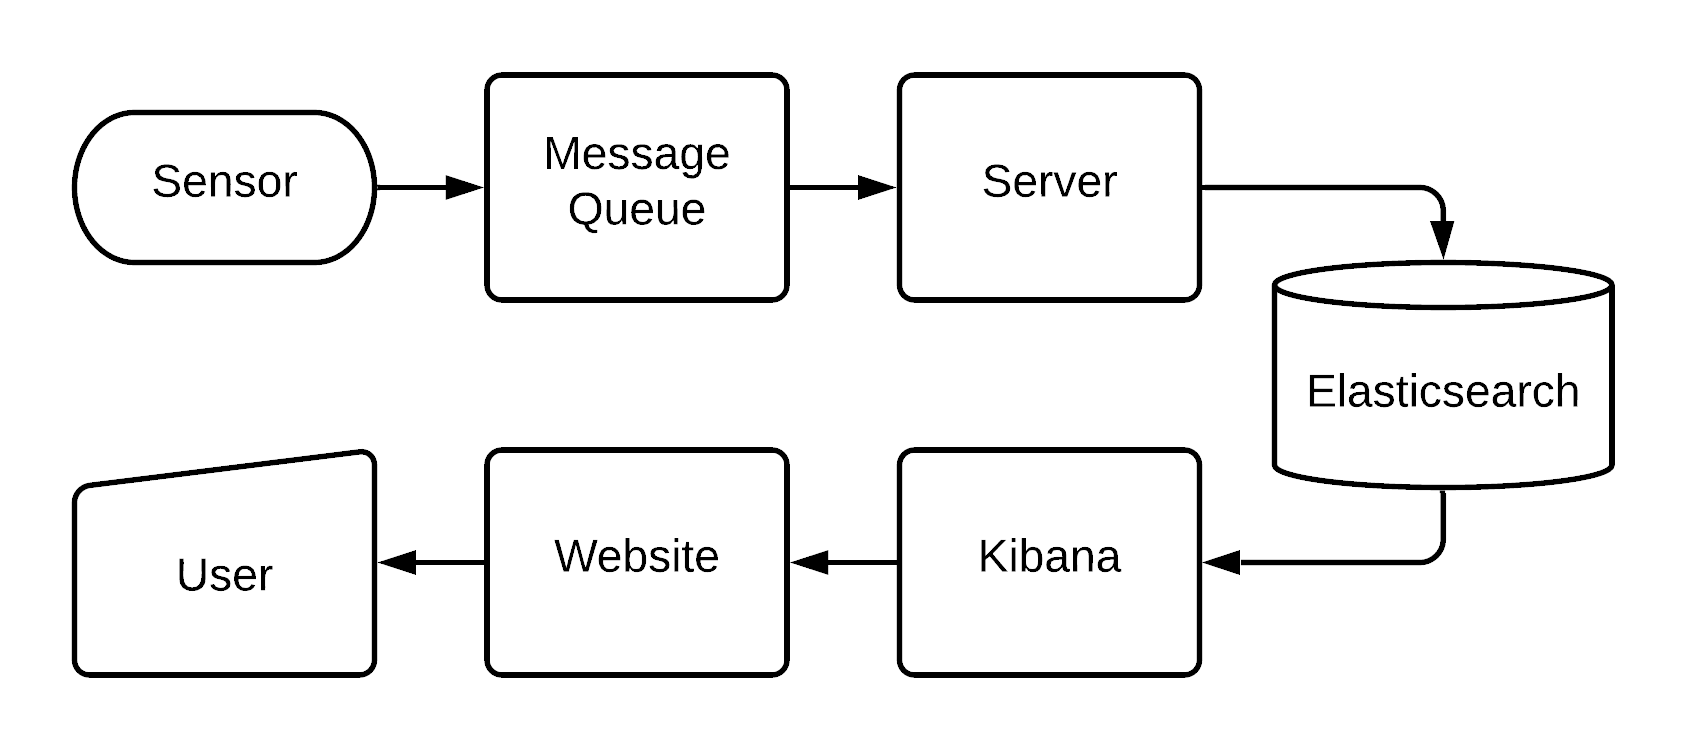
\includegraphics[width =\columnwidth]{dataflow.png}
  \caption{Data Flow Chart}
  \label{dataflow}
\end{figure}

\chapter{Implementation}

\section{Infrastructure Requirements}

\begin{table}[ht]
\label{hardware}
\begin{center}
\begin{tabular} {l|l|l} %left aligned
\hline
\hline
\textbf{Virtual Machine Instance} & \textbf{Operating System} & \textbf{Specifics}  \\
\hline
Data Ingestion Server & Debian 10 & 1 vCPU, 3.75 GB \\
ELK Server & Debian 10 & 1 vCPU, 3.75 GB \\
Frontend Server & Debian 10 & 1 vCPU, 3.75 GB \\
\hline 
\hline
\end{tabular}
\end{center}
\caption{Virtual Machine Details}
\end{table}


\section{Software Requirements}
Gunicorn was used as the production server for data ingestion.

\begin{table}[ht]
\label{software}
\begin{center}
\begin{tabular} {l|l} %left aligned
\hline
\hline
\textbf{Software Name} & \textbf{Version Number} \\
\hline
Gunicorn & 19.9.0 \\
Flask & 1.1.2 \\
Elastic Stack & 7.7 \\
OpenLayers & 6.3.1 \\
\hline 
\hline
\end{tabular}
\end{center}
\caption{Software Details}
\end{table}

Some of the softwares used in this project include Elastic stack(formerly known as ELK stack), 



\subsection{Elastic Stack}
Elastic Stack , formerly known as ELK stack is a group of open source products that help help users take data from any type of source and in any format and search, analyze, and visualize that data in real time. This can be deployed on the fully hosted and supported service by Elastic.org on their cloud service, ELK Cloud or as a standalone version on a local machine or a cloud service like this project does. 
\newline
\newline
Elastic Stack components:
\begin{enumerate}
    \item 
    Elasticsearch is a RESTful distributed search engine built on top of Apache Lucene and released under an Apache license. It is Java-based and can search and index document files in diverse formats.
    \item
    Logstash is a data collection engine that unifies data from disparate sources, normalizes it and distributes it. The product was originally optimized for log data but has expanded the scope to take data from all sources
    \item
    Beats are “data shippers” that are installed on servers as agents used to send different types of operational data to Elasticsearch either directly or through Logstash, where the data might be enhanced or archived.
    \item
    Kibana is an open source data visualization and exploration tool from that is specialized for large volumes of streaming and real-time data. The software makes huge and complex data streams more easily and quickly understandable through graphic representation
    
\end{enumerate}











\chapter{Results and Discussion}
Include tables (see Table \ref{XYComparison} for a template), figures and plots to represent your results if possible. What were the key outcomes? Do they match with expected results? Why/why not? Discuss and explain results where possible. Talk about challenges faced and the limitations of the present implementation if any. 
%template for table
\begin{table}[ht]
\label{XYComparison}
\begin{center}
\begin{tabular} {l|l|l} %left aligned
\hline
\hline
\textbf{Criteria} & \textbf{X} & \textbf{Y}  \\
\hline
A & B & C \\
D & B & C \\
\hline 
\hline
\end{tabular}
\end{center}
\caption{Comparison of  X and Y}
\end{table}

\chapter{Conclusions and Future Work}
\section{Conclusion}
Air quality and the state of the environment was and will continue to be an ever growing concern for mankind. This project will do it's part to help in the visualisation and analysis of air quality so that appropriate actions can be taken.
\section{Future Scope}
The possibilities of collaborations, future developments and improvements on this project are endless. Some of the future scopes for this include but are not limited to the following:
\newline
\begin{itemize}
    \item A customisable visualisation dashboard for the user to use
    \item Air quality prediction models that make smart predictions. 
    \item Mobile sensor technology mounted on vehicles 
    \item Route recommendation based on lesser pollution 
    \item Heat map based display for pollution comparison 

\end{itemize}



\bibliographystyle{ieeetr} 
\bibliography{bibmil.bib}
\appendix 
\chapter{sample appendix header 1}
%\label{app_1}
Appendices: 
Proofs, links to your code and any other misc. info that doesn't fit in nicely into other sections. 


\end{document}
